\section{eo\-Prop\-GAGen\-Op$<$ EOT $>$ Class Template Reference}
\label{classeo_prop_g_a_gen_op}\index{eoPropGAGenOp@{eoPropGAGenOp}}
$\ast$$\ast$$\ast$$\ast$$\ast$$\ast$$\ast$$\ast$$\ast$$\ast$$\ast$$\ast$$\ast$$\ast$$\ast$$\ast$$\ast$$\ast$$\ast$$\ast$$\ast$$\ast$$\ast$$\ast$$\ast$$\ast$$\ast$$\ast$$\ast$$\ast$$\ast$$\ast$$\ast$$\ast$$\ast$$\ast$$\ast$$\ast$$\ast$$\ast$$\ast$$\ast$$\ast$$\ast$$\ast$$\ast$$\ast$$\ast$$\ast$$\ast$$\ast$$\ast$$\ast$$\ast$$\ast$$\ast$$\ast$$\ast$$\ast$$\ast$$\ast$$\ast$$\ast$$\ast$$\ast$$\ast$$\ast$$\ast$$\ast$$\ast$$\ast$$\ast$$\ast$$\ast$$\ast$ eo\-Prop\-GAGen\-Op (for Simple GA, but Proportional) choice between Crossover, mutation or cloining with respect to given relatve weights  


{\tt \#include $<$eo\-Prop\-GAGen\-Op.h$>$}

Inheritance diagram for eo\-Prop\-GAGen\-Op$<$ EOT $>$::\begin{figure}[H]
\begin{center}
\leavevmode
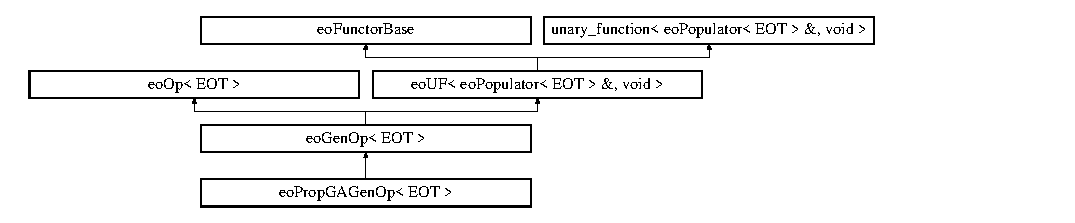
\includegraphics[height=2.54835cm]{classeo_prop_g_a_gen_op}
\end{center}
\end{figure}
\subsection*{Public Member Functions}
\begin{CompactItemize}
\item 
{\bf eo\-Prop\-GAGen\-Op} (double \_\-w\-Clone, {\bf eo\-Quad\-Op}$<$ {\bf EOT} $>$ \&\_\-cross, double \_\-w\-Cross, {\bf eo\-Mon\-Op}$<$ {\bf EOT} $>$ \&\_\-mut, double \_\-w\-Mut)\label{classeo_prop_g_a_gen_op_a0}

\begin{CompactList}\small\item\em Ctor from $\ast$ weight of clone $\ast$ crossover (with weight) $\ast$ mutation (with weight). \item\end{CompactList}\item 
virtual void {\bf apply} ({\bf eo\-Populator}$<$ {\bf EOT} $>$ \&\_\-pop)\label{classeo_prop_g_a_gen_op_a1}

\begin{CompactList}\small\item\em do the job: delegate to op \item\end{CompactList}\item 
virtual unsigned {\bf max\_\-production} (void)\label{classeo_prop_g_a_gen_op_a2}

\begin{CompactList}\small\item\em inherited from {\bf eo\-Gen\-Op}{\rm (p.\,\pageref{classeo_gen_op})} \item\end{CompactList}\item 
virtual std::string {\bf class\-Name} () const \label{classeo_prop_g_a_gen_op_a3}

\end{CompactItemize}
\subsection*{Private Attributes}
\begin{CompactItemize}
\item 
double {\bf w\-Clone}\label{classeo_prop_g_a_gen_op_r0}

\item 
{\bf eo\-Quad\-Op}$<$ {\bf EOT} $>$ \& {\bf cross}\label{classeo_prop_g_a_gen_op_r1}

\item 
double {\bf w\-Cross}\label{classeo_prop_g_a_gen_op_r2}

\item 
{\bf eo\-Mon\-Op}$<$ {\bf EOT} $>$ \& {\bf mut}\label{classeo_prop_g_a_gen_op_r3}

\item 
double {\bf w\-Mut}\label{classeo_prop_g_a_gen_op_r4}

\item 
{\bf eo\-Proportional\-Op}$<$ {\bf EOT} $>$ {\bf prop\-Op}\label{classeo_prop_g_a_gen_op_r5}

\item 
{\bf eo\-Mon\-Clone\-Op}$<$ {\bf EOT} $>$ {\bf mon\-Clone}\label{classeo_prop_g_a_gen_op_r6}

\end{CompactItemize}


\subsection{Detailed Description}
\subsubsection*{template$<$class EOT$>$ class eo\-Prop\-GAGen\-Op$<$ EOT $>$}

$\ast$$\ast$$\ast$$\ast$$\ast$$\ast$$\ast$$\ast$$\ast$$\ast$$\ast$$\ast$$\ast$$\ast$$\ast$$\ast$$\ast$$\ast$$\ast$$\ast$$\ast$$\ast$$\ast$$\ast$$\ast$$\ast$$\ast$$\ast$$\ast$$\ast$$\ast$$\ast$$\ast$$\ast$$\ast$$\ast$$\ast$$\ast$$\ast$$\ast$$\ast$$\ast$$\ast$$\ast$$\ast$$\ast$$\ast$$\ast$$\ast$$\ast$$\ast$$\ast$$\ast$$\ast$$\ast$$\ast$$\ast$$\ast$$\ast$$\ast$$\ast$$\ast$$\ast$$\ast$$\ast$$\ast$$\ast$$\ast$$\ast$$\ast$$\ast$$\ast$$\ast$$\ast$$\ast$ eo\-Prop\-GAGen\-Op (for Simple GA, but Proportional) choice between Crossover, mutation or cloining with respect to given relatve weights 



Definition at line 42 of file eo\-Prop\-GAGen\-Op.h.

The documentation for this class was generated from the following file:\begin{CompactItemize}
\item 
eo\-Prop\-GAGen\-Op.h\end{CompactItemize}
